% !TEX TS-program = pdflatexmk
% mnras_template.tex
%
% LaTeX template for creating an MNRAS paper
%
% v3.0 released 14 May 2015
% (version numbers match those of mnras.cls)
%
% Copyright (C) Royal Astronomical Society 2015
% Authors:
% Keith T. Smith (Royal Astronomical Society)

% Change log
%
% v3.0 May 2015
%    Renamed to match the new package name
%    Version number matches mnras.cls
%    A few minor tweaks to wording
% v1.0 September 2013
%    Beta testing only - never publicly released
%    First version: a simple (ish) template for creating an MNRAS paper

%%%%%%%%%%%%%%%%%%%%%%%%%%%%%%%%%%%%%%%%%%%%%%%%%%

\documentclass[a4paper,fleqn,usenatbib]{mnras}

\usepackage{newtxtext,newtxmath}
\usepackage[T1]{fontenc}
\usepackage{ae,aecompl}
\usepackage{graphicx}	% Including figure files
\usepackage{amsmath}	% Advanced maths commands
\usepackage{amssymb}	% Extra maths symbols
\usepackage{bm}

\newcommand{\nb}{n_{\rm b}}
\newcommand{\nc}{n_{\rm c}}
\newcommand{\ns}{n_{\rm s}}
\newcommand{\prob}{{\rm P}}
\newcommand{\normal}{{\rm{N}}}
\newcommand{\uniform}{{\rm U}}
\newcommand{\dirichlet}{{\rm D}}
\newcommand{\invwish}{{\rm W}^{-1}}
\newcommand{\alphas}{{\bm a}}
\newcommand{\specmean}{{\bm m}}
\newcommand{\speccov}{{\bm S}}
\newcommand{\classprob}{{p}}
\newcommand{\classprobs}{{\bm p}}
\newcommand{\objspec}{{\bm s}}
\newcommand{\objclass}{{\kappa}}
\newcommand{\objclasses}{{\bm \kappa}}
\newcommand{\objdata}{\hat{\bm d}}
\newcommand{\objnoise}{{\bm N}}
\newcommand{\scalemat}{{\bm \Gamma}}
\newcommand{\wfmean}{{\bm w}}
\newcommand{\wfcov}{{\bm W}}

%Editing commands
\newcommand{\bdw}[1]{\textbf{\textcolor{magenta}{BDW: #1}}}
\newcommand{\smf}[1]{\textbf{\textcolor{blue}{SMF: #1}}}
\newcommand{\mkn}[1]{\textbf{\textcolor{red}{MKN: #1}}}

%%%%%%%%%%%%%%%%%%%%%%%%%%%%%%%%%%%%%%%%%%%%%%%%%%

\title[Gaussian Process Spectra]{Gaussian Process Spectra}
\author[S. M. Feeney et al.]{
Stephen M. Feeney,$^{1}$\thanks{E-mail: sfeeney@flatironinstitute.org}
Benjamin D. Wandelt,$^{1,2,3,4}$
and Melissa K. Ness$^{1,5}$
\\
$^{1}$Center for Computational Astrophysics, Flatiron Institute, 162 Fifth Avenue, New York, NY 10010, USA\\
$^{2}$Sorbonne Universit\'e, CNRS, UMR 7095,  Institut d'Astrophysique de Paris (IAP), 98 bis boulevard Arago, 75014 Paris, France\\
$^{3}$Sorbonne Universit\'e, Institut Lagrange de Paris (ILP), 98 bis boulevard Arago, 75014 Paris, France\\
$^{4}$Department of Physics and Astronomy, University of Illinois at Urbana-Champaign, 1002 W Green St, Urbana, IL 61801, USA\\
$^{5}$Department of Astronomy, Columbia University, Pupin Physics Laboratories, New York, NY 10027, USA
}

% These dates will be filled out by the publisher
\date{Accepted XXX. Received YYY; in original form ZZZ}

% Enter the current year, for the copyright statements etc.
\pubyear{2019}

% Don't change these lines
\begin{document}
\label{firstpage}
\pagerange{\pageref{firstpage}--\pageref{lastpage}}
\maketitle

% Abstract of the paper
\begin{abstract}
This is a simple template for authors to write new MNRAS papers.
The abstract should briefly describe the aims, methods, and main results of the paper.
It should be a single paragraph not more than 250 words (200 words for Letters).
No references should appear in the abstract.
Context: Little empricial characterisation of information content in the spectra
Aims: Make models of the spectra to understand how spectral element features are correalted and how well we can predict missing parts of the spectra
Methods: Use Gaussian Process modeling
Results: Find that spectral absorption features of N elements are highly (but not perfectly) correlated by that all elements add additional information. Can use concert of measurements to predict missing very well
Conclusions :Use Gaussian process modeling to make first steps toward information content of element features. Futhermore we produce a generative model of the spectra and effectively de-noise to enable higher precision at lower SNR - important for optimising data and information extraction. 
\end{abstract}

% Select between one and six entries from the list of approved keywords.
% Don't make up new ones.
\begin{keywords}
keyword1 -- keyword2 -- keyword3
\end{keywords}

%%%%%%%%%%%%%%%%%%%%%%%%%%%%%%%%%%%%%%%%%%%%%%%%%%

\section{Introduction}

[Motivations/goals.] 


There is now a vast set of spectroscopic data and associated label data from surveys like APOGEE, GALAH, LAMOST, SEGUE and RAVE and an increasing number of large spectroscopic surveys will be starting observations in the coming years such as Sloan V, WEAVE, 4 MOST and Gaia RVS. Surveys like GALAH and APOGEE have revolutionised our empirical characterisation of the Milky Way and improved our understanding of its assembly, but both rely on expensive observations integrating to high signal to noise (up to SNR $>$ 100 per pixel) in the pursuit of precision abundances to provide optimal chemical differentiation across the sky (e.g. link to chemical tagging work). Surveys like Sloan V are obtaining an order of magnitude more stars via more efficient sky sampling and by relaxing the SNR limit to ~ 40 per pixel, yet at what precision expense in the derived labels like abundances? Furthermore, GAIA will deliver medium resolution spectra for 7 million objects, with N percent of this being at prohibitive signal to noise for abundance measurements given traditional approaches. There has been to date little characterisation of the true dimensionality and information content of the data. While surveys optimise their wavelength regions to attain an optimal number of element absorption features from which to make measurements, and aim for high signal to noise data, empirically the relationship between signal to noise, precision and information gain across a given wavelength region at a given resolution is unknown. Furthermore it is becoming clear that individual abundances can be measured from their impact on the entire spectral range (Ting 2018) and that precision abundances can be derived from very low resolution spectra (Ho et al., 2016). 
We are therefore at a point where we must assess what the information content of the spectral data actually is, and what expectations of  precision measurements we can make of the data, using automated and data-driven modeling techniques. What is empirically gained by adding an additional element of the same or different nucleosynthetic family in terms of additional spectral information? How correlated or anti-correlated are different spectral features in the data? With respect to the signal to noise required for precision abundance measurements, data-driven modeling like The Cannon and also The Payne have shown that the same precision can be obtained for APOGEE data with 1/4 to 1/9th of the observing time (1/2 to 1/3 of the SNR, so a SNR of around 40 compared to 100 for most abundances) and a precision near the theoretical limit (kramer-rao bound) can be obtained for APOGEE around a SNR of 40 (check), for most elements, which has motivated surveys like Sloan V to optimise their numbers of stars by collecting lower SNR data. Here we expand the 
examination of what information is in stellar spectra from an empirical standpoint. We investigate modeling the APOGEE spectral region using a Gaussian Process, creating a generative model which is an effective de-noising of the individual spectra, that can predict masked or missing spectral regions. We examine in detail the correlations between spectral pixels in element windows and the relative information gain attained by iterative abundance measurements. 

Our approach effectively pools information about stars. In doing this we can: 
% reorder this 
%1. correlations
%2. iformation content
%3. masked regions
%4. make a metric to demonstrate - denoised spectra so can quantify in a section In terms of variances []
%ratio of standard deviations of the pink to the grey
\begin{enumerate}
\item Predict masked (unmeasured or contaminated) regions of the spectra to make, e.g., abundance measurements that would otherwise be impossible. This may be particularly valuable in APOGEE for r-process element measurements where only one or two features exist from which to make measurements where this valuable element adds the dimensionality of the neturon-capture nucleosynthetic family [Section 2], or elements or features near the chip gaps that are present in some spectra and not others due to stellar velocities (citation. [Section 1] 
\item Examine in detail the empirical correlations in the spectra, make quantitative measurements of these correlations and identify in practice which elements are positively and which are negatively affiliated. [Section 2: might just want to add a plot of which are + and which are - correlated] 
\item Denoise to make precision measurements at lower SNR.  Generically, we can use the data-driven GP mixture model to denoise and thus enhance the data, potentially enabling new discoveries. This should work for high S/N and low S/N regions; how useful this is depends on the size of the effects we may want to discover. Our expectation is that this is particulalry good for very weak features such as (Hasselquist) expectation is can do a lot better with abundance measurements, similarly to that previously demonstrated with generative modeling (The Cannon, The Payne). 
\item Determine the most informative regions of spectra and make a measure of the information content of the data to, e.g., determine whether we can retain sensitivity to abundances by observing a reduced spectral range and to understand if we have a set of N elements measured, do we gain information empirically by moving to N+1 measurements, for different element combinations, at the SNR of the APOGEE data. 
\end{enumerate}

%Is there any purpose of measuring all these elements? Empirically extra information in them? 

%-first look at the information content of the spectra
%-first characterisation and mapping of the element correlations

%state just red clump sample 

%[Ce, Cu, Mg, Ni, Mn, N, C, Ti, Si, Mg, Na, Fe, O, Ti, Ca, Nd, Fe, Si, Mn, Al, N, Ni, C]
%light: C, N
%light odd-Z: Na, Al
%alpha: Mg, Ti, Si, O
%iron-peak: Cu, Ni, Mn, Fe
%neutron capture r-process: Ce, Nd



%Fig 4 - trying to bring out the correlation structure in a slightly different way

%Fig 4 - perfectly uncorrelated would be random purpose and yellow because none of the pixels in the bin compare about any of the pixels in any other bin. If perfectly correlated yellow all up the top, purple all down the bottom. 

%-not parameterised in any physical way
%understanding of stellar spectra is truly rudimentary 
%this is part of a bigger effort in order to (under the assumption that everything is Guassian) allows us to learn the covariance at every point completely independent of any given physical template. 
%- question about the degrees of freedom (N*N)/2 degrees of freedom, diagonal of the covariance matrix
%- big thing is it shows the covariances
%-understand what the information content of the spectra%
%-inferring true spectra of every star.( N*N + Nclasses*2 + N*N)/2
%in the context of a much more sophistocated model 
%-runs into problems as matrix algebra (just gets really slow) 
%-new things
%-can do de-noising 

%Fig 6: information gain for each element and then pick the one that is most informative and then calculate the information gain on the window of interest given most informative element and each other one
%-log of the determinant of the covariance matrix of the window/ log of the covariance matrix of the window conditioned on other data
%-



%to do: For the Figure 6 - a list of the windows and the element families and then that is a whole little section . 

%Fig 2 - go down to just the window

%Fig 5: corner put SNR 

%state just red clump sample 

%How will we do this? By modeling the spectra as a data-driven Gaussian Process. What is a GP and what are relevant applications.

%%%%%%%%%%%%%%%%%%%%%%%%%%%%%%%%%%%%%%%%%%%%%%%%%%




\section{Data} 

For our modeling we use the APOGEE red clump spectra from DR14 (cite Majewski, and Bovy 2014). These spectra comprise $29502$ stars with a mean SNR of XX and range of SNR of 20-XX.  The contamination of red giant stars within this sample is on the order of 5-20 percent (Bovy, Ting).  These make an ideal test case for our modeling being restricted in their range of effective temperature and surface gravity so we can assume that our overall measurements are driven by abundance variations and not systematic variations across stellar parameters. The metallicity range of the red clump stars span --1.0 $<$ [Fe/H] $<$ 0.5 and they are distributed from R$_{GAL}$ = 4 to 20 kpc. 


The data have been downloaded from the APOGEE database and come radial velocity shifted and continuum-normalised (with a slight SNR dependence on the continuum normalisation that we discover with our Gaussian Process modeling. The spectra cover the range 15100.80-16999.81 \AA, using $\nb = 8575$ spectral bins. 

\section{Methods}

Describe Gaussian Process. True spectrum for each star is drawn from a GP with a mean spectrum and covariance matrix to be inferred from the data. We do not assume a kernel for our GP covariance, but rather infer the correlations between the observed spectral bins. This is so we can model the exact covariance and not worry about suboptimal choices of kernels caused by non-stationarity or different correlation lengths, line shapes, etc. The main downside of doing this is we can not make predictions for the spectra between the observed bins, though we could, given data observed on shifted or irregularly or different-spaced grids. We assume uninformative priors on the mean and covariance. We adopt an infinite uniform prior on the mean and a Jeffreys prior on the covariance matrix (precise form in notes).

Data are observed with Gaussian noise that is uncorrelated between spectral bins; masked pixels are assigned unit flux and effectively infinite noise uncertainties. These data, the inferred parameters, the likelihood and priors would fully specify the model if we had only one class. To account for the fact that the red clump might consist of multiple distinct populations (or one population whose distribution of true spectra is non-Gaussian) we allow for multiple classes to exist in our model. In this instance, each star is also assigned membership to a particular class. Class memberships are drawn from categorical distributions, with class probabilities drawn from a symmetric Dirichlet prior with concentration parameter $\alpha=1$.

The network diagram for our hierarchical Bayesian model is shown in Fig.~\ref{fig:network_diagram}, with the parameters, data and constants described in Table~\ref{tab:params} and the probability distributions defining each link set out in Table.~\ref{tab:prob_dists}. The particular set of probability distributions chosen allow for the conditional distributions of each latent variable to be written analytically, and we hence use Gibbs sampling~\cite{Geman_and_Geman:1984Geman_and_Geman:1984} to estimate the joint posterior.

\begin{figure}
	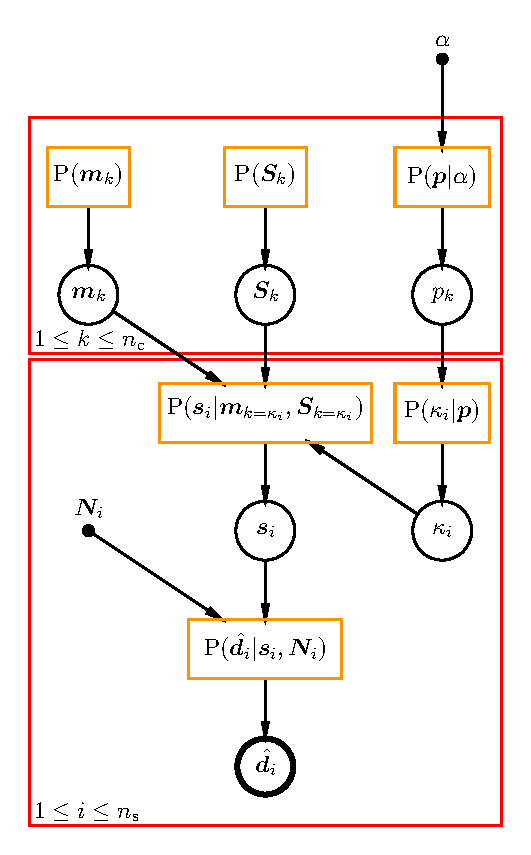
\includegraphics[width=\columnwidth]{bhm_plot.pdf}
    \caption{Network diagram for our hierarchical Bayesian model which is a graphical representation of our implemented modeling of the data. See Table 1 for the parameter descriptions.}
    \label{fig:network_diagram}
\end{figure}
%what all parameters are, what all of the observables are and what the relationships are between the two
%table 1 and Figure 1 set out all of the probability distributions that describe the model
%the second part of Table 1 sets out the conditional distributions that you need to perform Gibbs sampling.  


\begin{table}
    \centering
    \caption{Model parameters, data and constants.}
    \label{tab:params}
    \begin{tabular}{ll}
        \hline
        quantity & description \\
        \hline
        $\ns$ & number of stars (29502) \\
        $\nc$ & number of classes (default: 1) \\
        $\nb$ & number of spectral bins (default: 343) \\
        $\specmean_k$ & mean spectrum of $k^{\rm th}$ class \\
        $\speccov_k$ & intrinsic spectral covariance of $k^{\rm th}$ class \\
        $\classprob_k$ & $k^{\rm th}$ class probability: fraction of stars in $k^{\rm th}$ class \\
        $\alpha$ & concentration parameter of Dirichlet prior on class fractions \\
        $\objspec_i$ & true spectrum of $i^{\rm th}$ star \\
        $\objclass_i$ & class assignment of $i^{\rm th}$ star \\
        $\objdata_i$ & observed spectrum of $i^{\rm th}$ star \\
        $\objnoise_i$ & noise covariance matrix of $i^{\rm th}$ star \\
        \hline
    \end{tabular}
\end{table}


\begin{table*}
    \centering
    \caption{Priors, likelihoods and conditional distributions for Gibbs sampling. In our simplified notation, $\uniform$, $\dirichlet$, $\normal$ and $\invwish$ denote uniform, Dirichlet, normal and inverse-Wishart distributions, respectively.}
    \label{tab:prob_dists}
    \begin{tabular}{lll}
        \hline
        distribution & form & process \\
        \hline
        $\prob\left(\specmean_k\right)$ & $\uniform\left(-\infty,\infty\right)$ & Prior on $k^{\rm th}$ class's mean spectrum \\
        $\prob\left(\speccov_k\right)$ & $\left| \speccov \right|^{-\left(\nb+1\right)/2}$ & Prior on $k^{\rm th}$ class's spectrum covariance \\
        $\prob\left(\classprobs|\alpha\right)$ & $\dirichlet\left(\alpha\right)$ & Prior on class probabilities \\
        $\prob\left(\objspec_i|\specmean,\speccov,\objclass_i\right)$ & $\normal\left(\specmean_{k=\objclass_i},\speccov_{k=\objclass_i}\right)$ & $i^{\rm th}$ object's spectrum as Gaussian Process \\
        $\prob\left(\objclass_i = k|\classprobs\right)$ & $\classprob_k$ & $i^{\rm th}$ object's class membership \\
        $\prob\left(\objdata_i|\objspec_i,\objnoise_i\right)$ & $\normal\left(\objspec_i,\objnoise_i\right)$ & Noisy, masked spectral measurements \\
        \hline
        $\prob\left(\specmean_k | \speccov_k, \objspec, \objclasses \right)$ & $\normal \left( \frac{1}{n_k} \sum_{\objclass_i = k} \objspec_i, \frac{1}{n_k} \speccov_k \right)$ & Conditional on $k^{\rm th}$ class's mean spectrum \\
%        $\prob\left(\speccov_k | \specmean_k, \objspec, \objclasses \right)$ & $\left| \speccov_k \right|^{-(n_k + \nb + 1)/2} \exp \left( -\frac{1}{2} {\rm tr} \left[ \scalemat_k \speccov_k^{-1} \right] \right)$, where & Conditional on $k^{\rm th}$ class's spectrum covariance \\
        $\prob\left(\speccov_k | \specmean_k, \objspec, \objclasses \right)$ & $\invwish \left(n_k, \scalemat_k \right)$, & Conditional on $k^{\rm th}$ class's spectrum covariance \\
         & where  $\scalemat_k = \sum_{\objclass_i = k} \left( \objspec_i - \specmean_k \right) \otimes \left( \objspec_i - \specmean_k \right)$ & \\
        $\prob\left(\classprob_k | \objclasses, \alpha\right)$ & $\dirichlet\left(\alphas\right)$, where $a_k = \alpha + n_k$ & Conditional on class probabilities \\
        $\prob \left( \objspec_i | \specmean_{k=\objclass_i}, \speccov_{k=\objclass_i}, \objdata_i, \objnoise_i \right)$ & $\normal \left( \wfmean_i, \wfcov_i \right)$, & Conditional on $i^{\rm th}$ object's spectrum \\
         & where $\wfcov_i = \left( \speccov_{k=\objclass_i}^{-1} + \objnoise_i^{-1} \right)^{-1}$ &  \\
         & and $\wfmean_i = \wfcov_i \left( \speccov_{k=\objclass_i}^{-1} \specmean_{k=\objclass_i} + \objnoise_i^{-1} \objdata_i \right)$ &  \\
        $\prob \left( \objclass_i = k | \specmean, \speccov, \classprobs \right)$ & $ \frac{ \exp \left( -\frac{1}{2} \left[ \chi^2_{i,k} + \ln \left| \speccov_k \right| \right] + \ln \classprob_k \right) }{ \sum_{k^\prime} \exp \left( -\frac{1}{2} \left[ \chi^2_{i,k^\prime} + \ln \left| \speccov_{k^\prime} \right| \right] + \ln \classprob_{k^\prime} \right) }$, & Conditional on $i^{\rm th}$ object's class membership \\
         & where $\chi^2_{i,k} = \left( \objspec_i - \specmean_k \right)^T \speccov_k^{-1} \left( \objspec_i - \specmean_k \right) $ &  \\
        \hline
    \end{tabular}
\end{table*}

%%%%%%%%%%%%%%%%%%%%%%%%%%%%%%%%%%%%%%%%%%%%%%%%%%

We take the 29502 red clump stars identified in the APOGEE dataset with their $\nb = 8575$ spectral bins over the range 15100.80-16999.81 \AA. Inversion of the resulting $\nb \times \nb$ covariance matrices would be too slow to permit inference, and we thus restrict our analysis to a set of spectral windows centred on lines confidently assigned to individual elements. These element windows have been chosen from the set of windows used to drive the APOGEE abundances (described in citation). Specifically, we process all spectral bins within $\pm 1.5$ \AA\ of the line centres tabulated in Table~\ref{tab:window_centres}, reducing the number of spectral bins to $\nb = 343$ and hence inversion time by a factor of $\sim15000$. These spectral windows were selected using the APOGEE line list and communication with Jon Holtzman and Matthew Shetrone \citep{Holtz2015}. 

\begin{table}
    \centering
    \caption{The list of the 25 elements that we select for our spectral modeling and their corresponding central wavelength (in a vacuum) corresponding to Figure 4.}
    \label{tab:window_centres}
    \begin{tabular}{lc}
        \hline
        element & window centre / \AA \\
        \hline
        Al & 16723.500 \\
        C & 15582.101 \\
        Ca & 16155.176 \\
        Ce & 15789.063 \\
        Co & 16158.700 \\
        Cr & 15684.264 \\
        Cu & 16010.023 \\
        Fe & 15495.100 \\
        Ge & 16764.238 \\
        K & 15167.081 \\
        Mg & 15745.000 \\
        Mn & 15221.867 \\
        N & 15321.871 \\
        Na & 16378.276 \\
        Nd & 15372.342 \\
        Ni & 15559.517 \\
        O & 15760.300 \\
        P & 15715.930 \\
        Rb & 15293.534 \\
        S & 15482.319 \\
        Si & 15964.600 \\
        Ti & 15339.241 \\
        V & 15929.052 \\
        Y & 15624.142 \\
        Yb & 16502.973 \\
        \hline
    \end{tabular}
\end{table}

%%%%%%%%%%%%%%%%%%%%%%%%%%%%%%%%%%%%%%%%%%%%%%%%%%

\section{Results}

\subsection{Validation of Methodology: Predicting Unmeasured Spectral Regions}

To avoid the complications of comparing data gathered by different spectrographs we validate our model and code by artificially masking a portion of one of our APOGEE spectra, namely the 15789 \AA\ Cerium (Ce II) window of our lowest-SNR star (2M18335753-1302240), with an SNR measurement of 21 as listed in the APOGEE allStar file. 


We select the Ce II line because it is a high-value detection in the APOGEE spectra region. This identification (Cuhna+ 2017) and subsequent validation of the prospect of making measurements from this line has added the prospect of examining the s-process enrichment in the APOGEE survey, building on its reach and power in mapping the alpha, light and iron-peak elements across the disk and into the halo and local group (Majewski, Hayden, Nidever, Weinberg). Nine windows were identified in Cuhna et al., 2017 and we select one (unblended) Ce II window here (the line centered on 15784.75 \AA\ in air, converted to the vacuum scale of the APOGEE spectra, for validation of our methodology. 


The measured data for this star are plotted in Figure~\ref{fig:recovery_test} as a solid black line, with the artificially masked region picked out as a dashed line. The 68\% credible interval for the posterior probability on the star's true spectrum is plotted as dark grey, with the corresponding prediction for the observed spectrum (which also takes into account the uncertainty on the observations) plotted in light grey. This prediction (the posterior predictive distribution of the measured data) is in excellent agreement with the measured data, indicating that our model is capable of inpainting masked regions without bias. Note, in addition, that the uncertainty on the generated spectrum is much smaller than the measurement noise, demonstrating our method's ability to de-noise observed spectra.

This de-noising property is relevant in the regime of extracting information from both weak lines and lower signal to noise data than typically or previously required. In addition to the neuron capture element, Cerium, the APOGEE spectral region has been shown to contain a number of Neodymium (Nd II) lines, which Hasselquist et al., 2016 estimates is detectable in $\approx$ 18 percent of APOGEE spectra, using equivalent width fitting techniques. Our expectation is this fraction will vastly improved given our Gaussian process modeling of the spectral lines which, similarly to our demonstration of the Ce line, can generate a spectral model with lower uncertainty than the measurement noise. \mkn{SF: can you check I am saying this the right way, let's also point out the SNR of the star that we have Ce and Nd detections later on in the text.}

\begin{figure}
	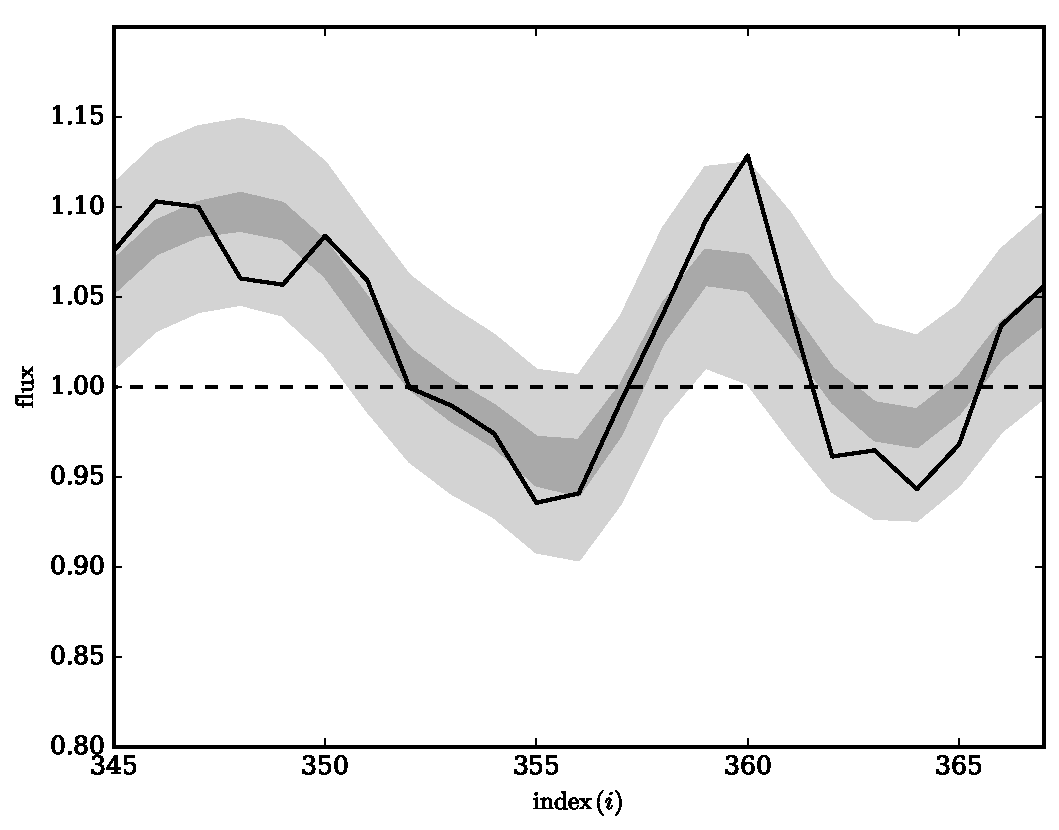
\includegraphics[width=\columnwidth]{apogee_centers_final_29502_spc_rec_test_recovery_zoom.pdf}
    \caption{This Figure shows the validation of the model and the method showing the recovery of an artificially masked portion of the spectra. This $\approx$ 22 \AA\ region of spectra is centered on Cerium line with a central wavelength of 15789 \AA\ (see Table 1). We select a star with a SNR of 21 for this demonstration of our model recovery, to highlight the performance of the model even for very low SNR data. The inferred spectrum is shown in the dark-grey shaded region and the measured spectra is shown in the solid black line. The model is in excellent agreement with the data once noise is taken into account (light-grey shaded region).}
    \label{fig:recovery_test}
\end{figure}

\subsection{APOGEE Inference: Feature Correlations Across the Abundance Windows}


Our inference produces samples of the probability, mean spectrum and covariance matrix for each class considered, and the true spectrum and class membership of each object. Focusing initially on the single-class case, we plot our covariance and mean inference in Figures~\ref{fig:inferred_cov} and~\ref{fig:gp_reals}, respectively. We plot the mean-posterior covariance matrix in Figure~\ref{fig:inferred_cov} (left panel). The covariance has strong off-diagonal structure, indicating that certain spectral features are highly correlated and anti-correlated ({\bf discuss potential kernel choices?}). Its eigenspectrum also decays rapidly: only 241 of 557 eigenmodes have eigenvalues larger than 1/100 of the maximum. A low-rank approximation to the mean covariance retaining only these eigenmodes is plotted in the centre panel of Figure~\ref{fig:inferred_cov}, and the resulting residuals (multiplied by a factor of 500 to render visible) in the right panel. Exploiting this decaying eigenspectrum by assuming the covariance is rank deficient would greatly reduce computation time (by a factor of roughly 12 if 241 modes were retained). Na\"ively projecting the data onto the largest principal components of the sample covariance matrix prior to inference severely degrades performance. Modifying the hierarchical model (along the lines of {\bf citations}) to explicitly infer a rank-deficient covariance matrix is left to future work.

\begin{figure*}
	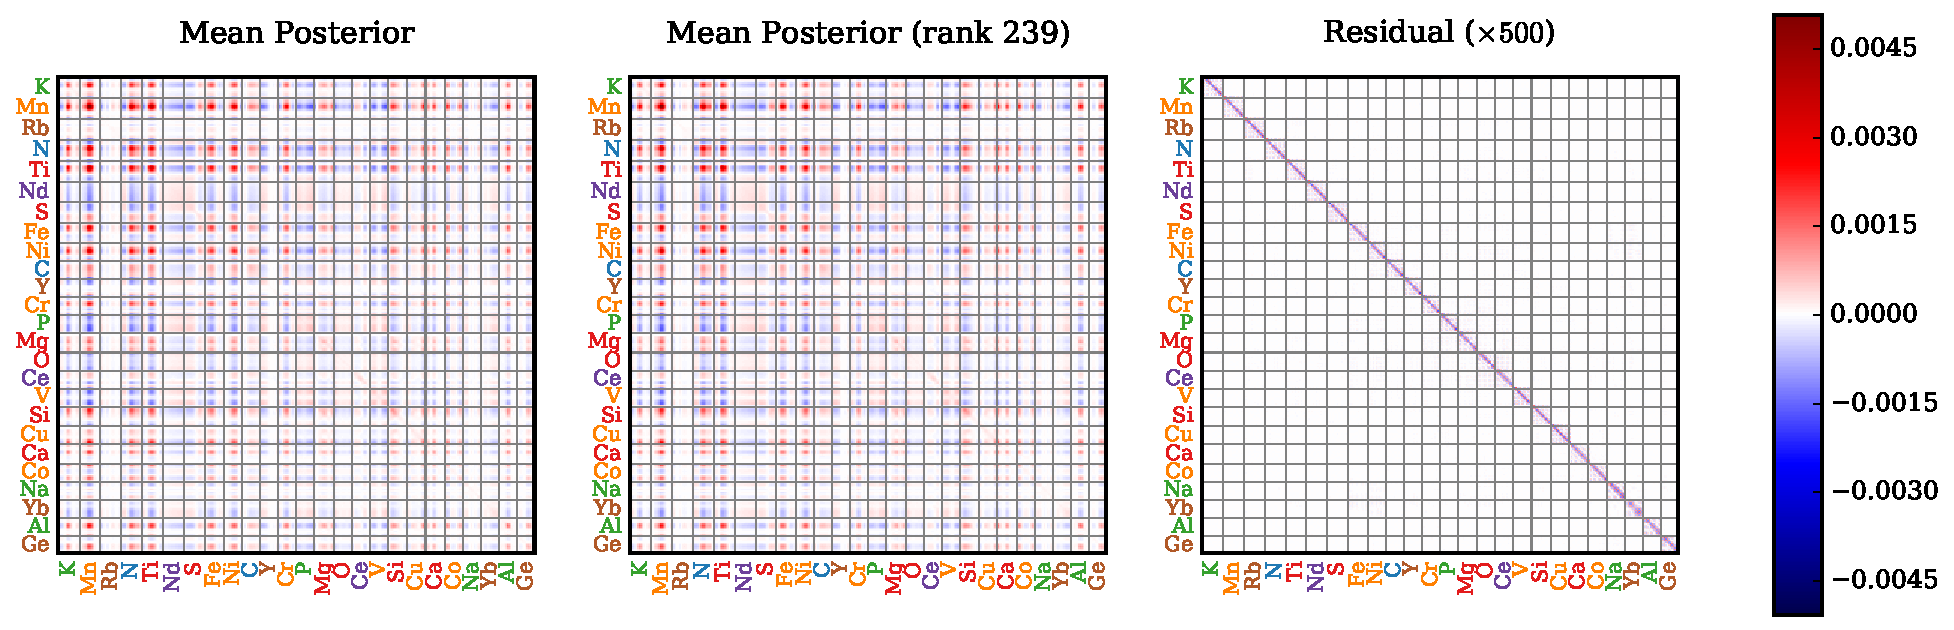
\includegraphics[width=2\columnwidth]{apogee_centers_final_29502_spc_win_wid_1p5_low_rank_covariance.pdf}
    \caption{At left, the mean-posterior covariance matrix of the 343 spectral pixels that we model, with the corresponding colour bar giving the magnitude of this covariance at far right (in units of flux$^2$). The divergent colour map shows the most positive and negative covariances in red and blue respectively and zero covariance as white. This matrix demonstrates that the spectral pixels are highly correlated. The middle panel shows the reduced-rank approximation of the full covariance matrix, constructed from all eigenvectors of the estimate of the mean covariance matrix, including the eigenvalues within $10^{-4}$ of the largest. This represents a 30 percent reduction in the number of pixels used to build the mean posterior. The residual ($\times$ 500) of the mean posterior and reduced rank posterior is shown in the panel at far right.  The non-zero diagonal term represents that the variance of the data is (marginally) not entirely conserved in the rank reduction. }
    \label{fig:inferred_cov}
\end{figure*}
% to try to demonstrate how many 
% can speed things up in the inference by reducing the rank of the covariance matrix which is a 30 percent reduction in the number of pixels. 
%reduced rank puts null modes in the matrix - all structure in residuals is india
% the low rank version is missing variance on the diagonal 

\begin{figure*}
	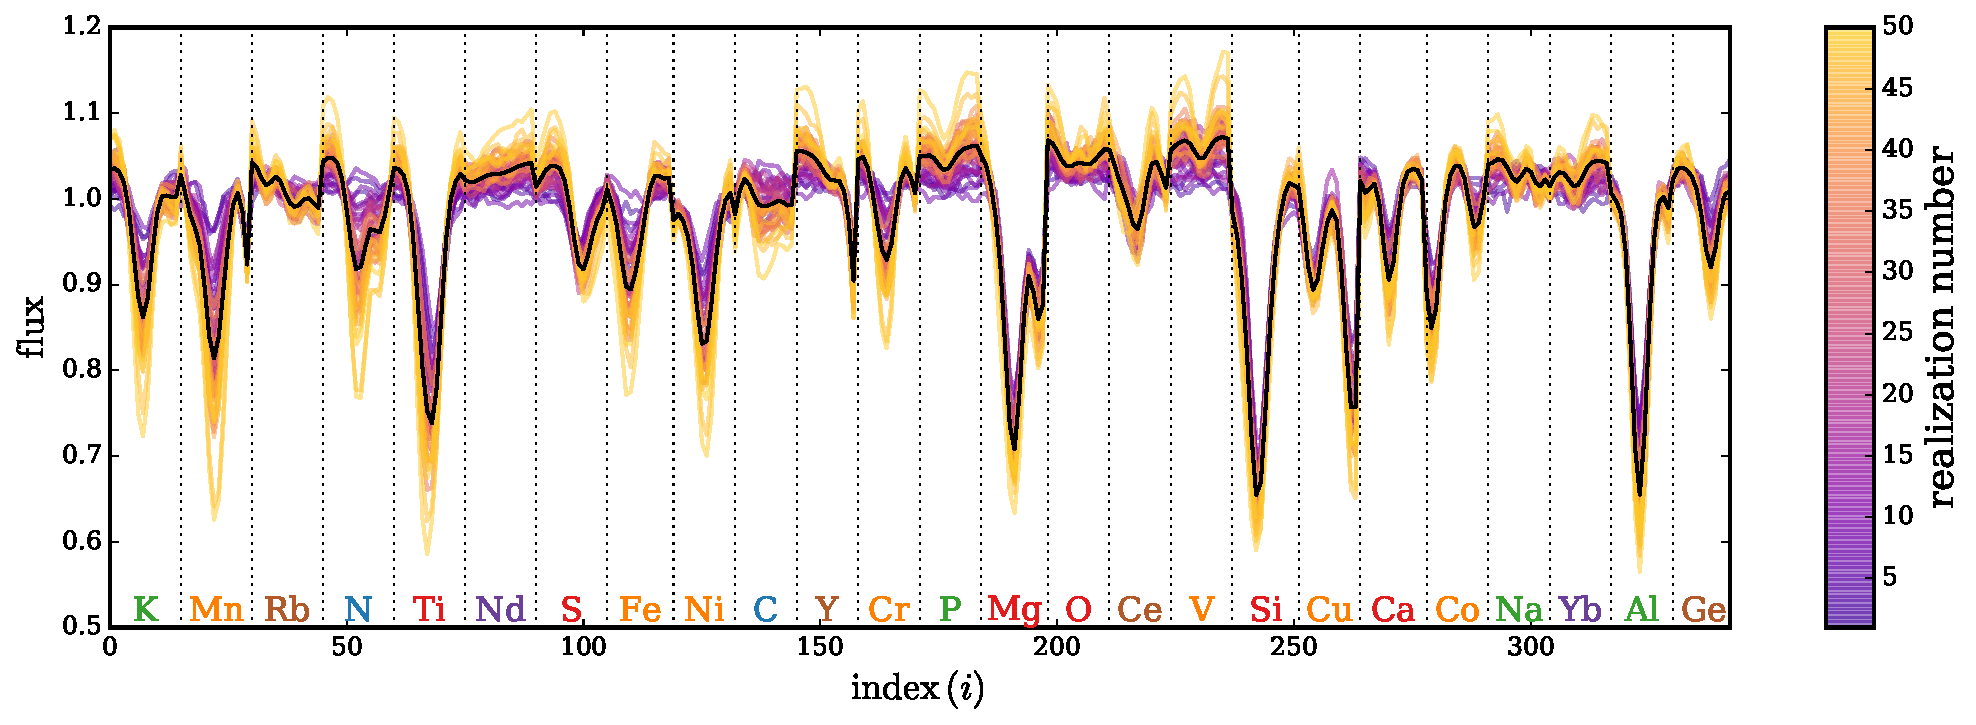
\includegraphics[width=2\columnwidth]{apogee_centers_final_29502_spc_win_wid_1p5_gp_realizations.pdf}
    \caption{The mean-posterior mean spectrum of our Gaussian process model is shown in black. A sample of 50 individual realizations drawn from our Gaussian Process model fit using the APOGEE data is shown coloured from purple to yellow, according to the measured flux in the first spectral bin. The color scale is shown at right. The coloured realisations are a complement to Figure 3 in that they are demonstrative of how correlated the pixels are. Entirely uncorrelated data would show no gradient structure in the color of the realisations whatsoever. We see a clear stratification of yellow to purple as  function of the flux magnitude for most of the pixels. \textcolor{blue}{add colorbar}}
    \label{fig:gp_reals}
\end{figure*}

%using samples of covariance matrix and samples of sample posterior you can draw examples of the spectra itself 
%samples of mean and covariance and pick a randomly chosen sample and draw a realisation of that Gaussian process from that mean and covariance. 
%mean spectrum m (posterior) and some covariance s and then have samples of those; black ine is the sum over i of the m/i 
%realisations are gaussian with mean of mi and covafaince si) 
%m$_i$, s$_i$, \specmean = \frac{\sum{i=1}{n}}{m_i}{n}; r $\sim$ N(\specmean_i, \speccov_i) 
%\specmean\ and \speccov

The posterior mean of the mean spectrum is plotted in black in Figure~\ref{fig:gp_reals}. The mean spectrum is extremely well constrained: its 68\% credible interval is narrower than the width of line. To illustrate the covariance structure captured by our model, we overlay 50 realizations drawn from our Gaussian-Process model conditioned on the APOGEE data, colour-coded by the value they take in the first spectral bin. These samples can be interpreted as examples of potential noiseless true spectra that could have led to the data. They illustrate the variability permitted by the model and highlight certain clear trends, most notably highly correlated differences in line depths.

We demonstrate our inference of the true spectra of individual stars in Figure~\ref{fig:inpainting_denoising_examples}, selecting six illustrative examples. From top to bottom, we pick out two spectra whose 15789 \AA\ Cerium windows are completely masked; two spectra whose 16058 \AA\ Neodymium windows are fully masked; and the two lowest signal-to-noise spectra. The APOGEE IDs for these stars are 2M00014650+7009328, 2M00031631+0042234, 2M04480027+3337594, 2M06053121-0631412, 2M18335753-1302240 and 2M18295507-0340512, with signal-to-noise ratios of 49, 63, 75, 41, 21 and 23. Each panel of Figure~\ref{fig:inpainting_denoising_examples} contains two shaded regions. The pink shaded area indicates the one-sigma deviations from the measured spectra due to noise (these are infinitely wide when the spectrum is masked); the grey, the 68\% posterior credible intervals on the true spectra. Recall that we are inferring the true spectra only at the measured spectral bins only. In this sense the smooth grey curves are perhaps misleading, as the posterior uncertainty is strictly infinite between datapoints.
 
true spectra. fit to observations. inpainting, denoising. quantify? any underperformance? Ni band of star 2. N/Mn (and Ti) bin of lowest SNR star (and 2nd lowest?).
number of classes, high-dim inference

\begin{figure*}
	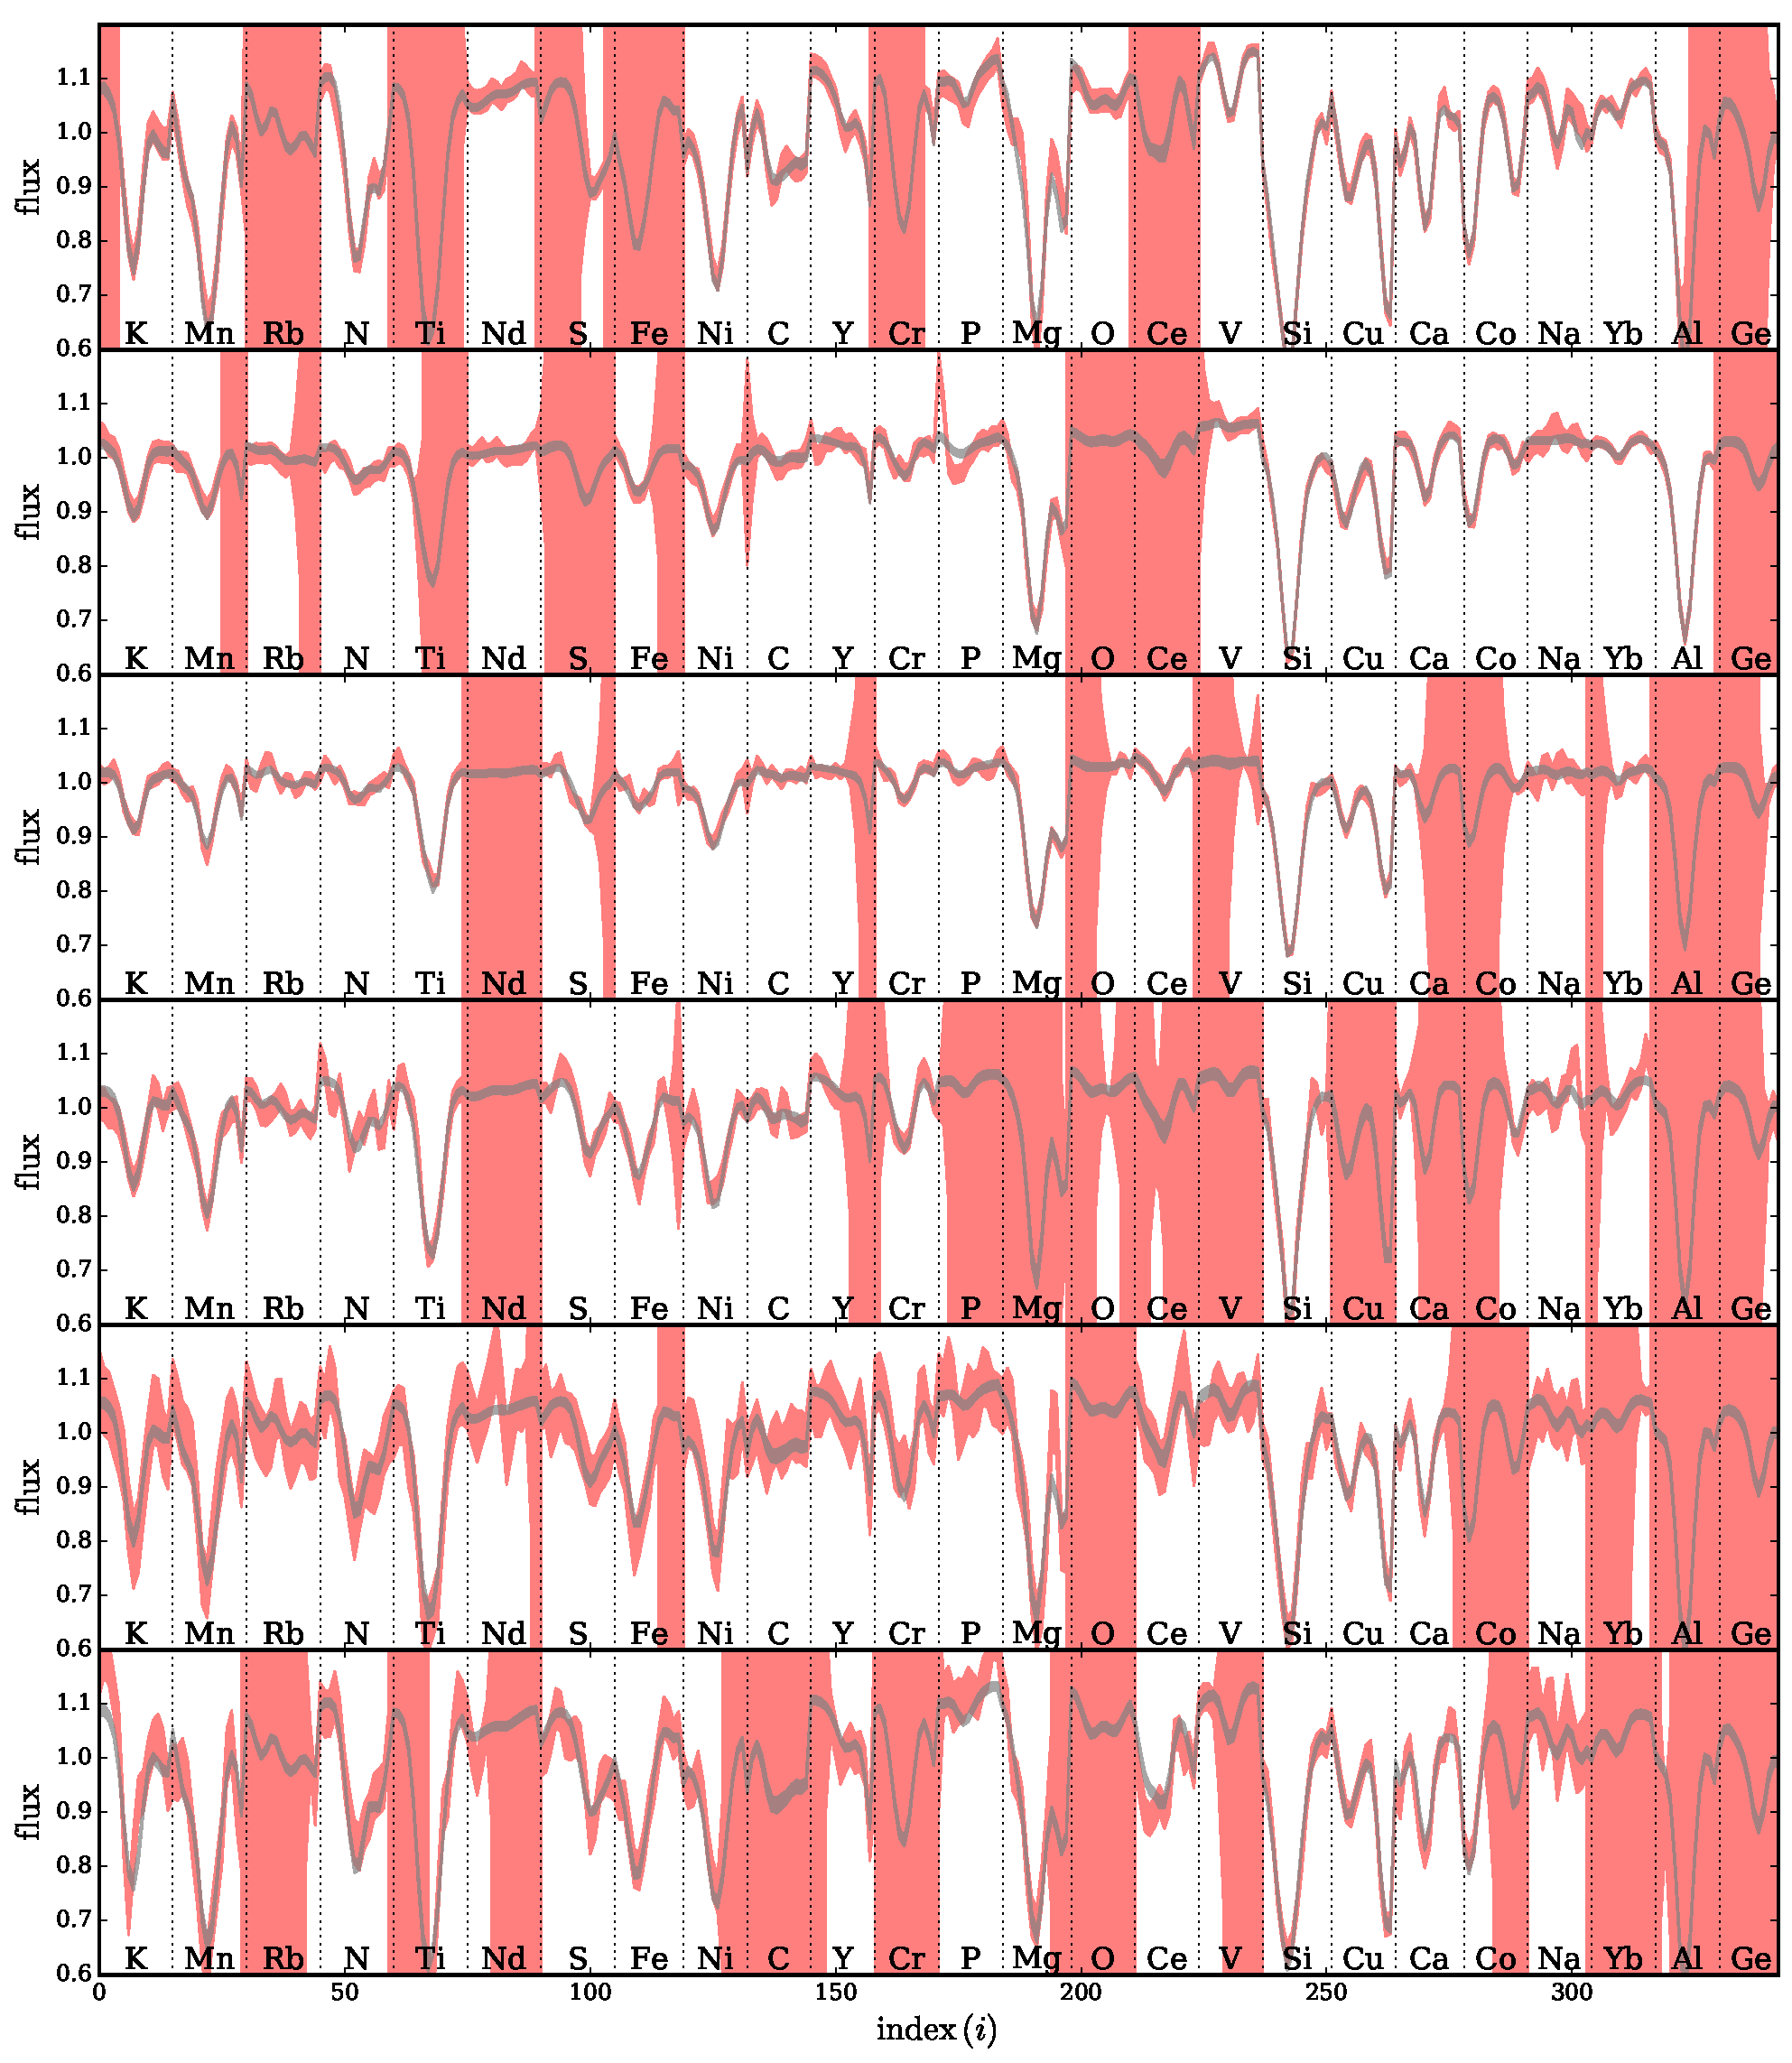
\includegraphics[width=2\columnwidth]{apogee_centers_final_29502_spc_win_wid_1p5_save_spectra.pdf}
    \caption{This Figure shows 6 unique stars, all with low SNR, as demonstrative of our modeling capabilities in the realm of relatively poor data quality, to both inpaint and denoise the data. From top to bottom, the SNR of the stars are 49, 63, 75, 41, 21 and 23, respectively. The observed spectra is shown as the pink shaded regions (note the masked regions in the APOGEE spectra where data is missing for these stars) and the inferred ``true'' spectra from the model is shown in the grey shaded regions. There is excellent agreement between the model and data.  The spectral regions shown are our 25 elements from Table 1, centered at the centre wavelength of each element, with a bandwidth of $\pm$ 2.5 \AA. Note that the first two spectra have masked Cerium lines centered on 15789 \AA\, where the model infers the line profiles which could in principle be used to return a Cerium abundance for these stars. The middle two stars have the Neodymium line centered on 16058 \AA\ masked and here the model infers very weak line profiles at this central wavelengths, which renders recovery of this abundance unlikely (and across all SNR examined in this Figure). All other lines inferred by the model are essentially denoised versions of the spectra from which higher precision abundances can be in principle determined compared to using the originally observed spectra itself. }
    \label{fig:inpainting_denoising_examples}
\end{figure*}

\subsection{The Measured Information Content in the Spectra}



predictivity
Here we measure information gain. Given one element, how much information do we gain by measuring one more element, and then another. Importantly, we have the caveat that this is for elements measured from these particular spectral regions, could change as a function of some lines. 
Demonstrate for each family
Metric is this: 
What we find is essentially every single element adds information. Flat line would indicate no additional information, falls of exponentially at different rates for all the elements. Log scale so fractional gain for first N elements is XX and fractional gain for elements $>$ 5 is XX percent, relatively independent of which element is conditioned on. 

\begin{figure*}
	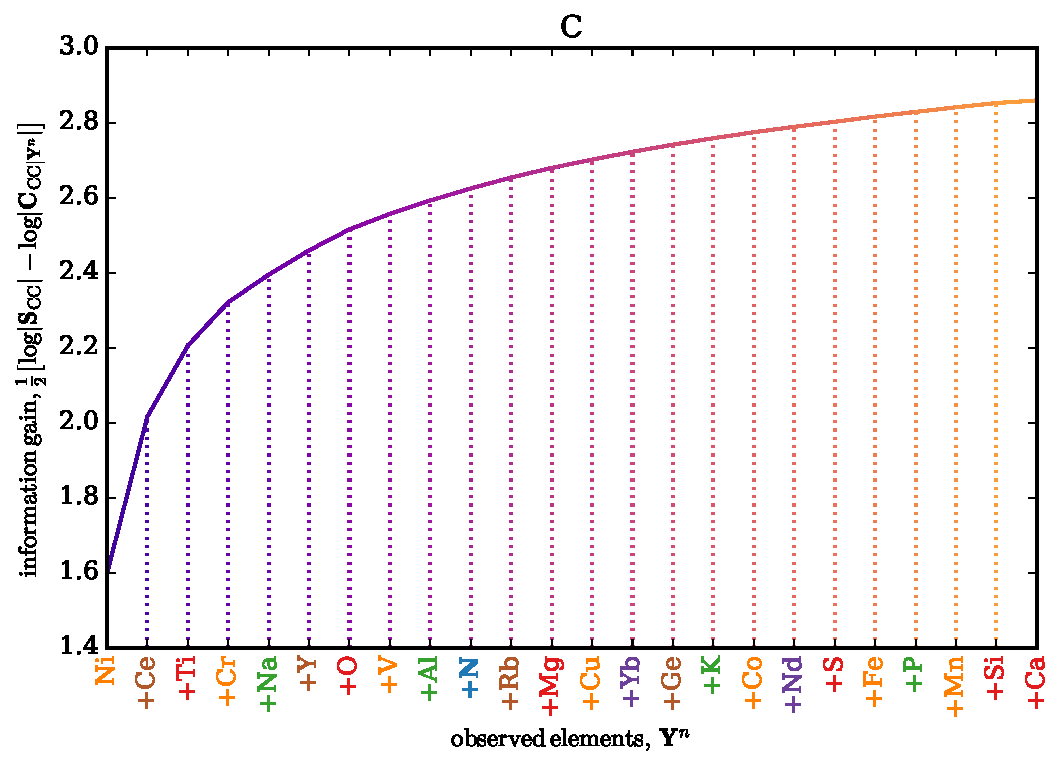
\includegraphics[width=\columnwidth]{apogee_centers_final_29502_spc_win_wid_1p5_c_inf_gain.pdf}
	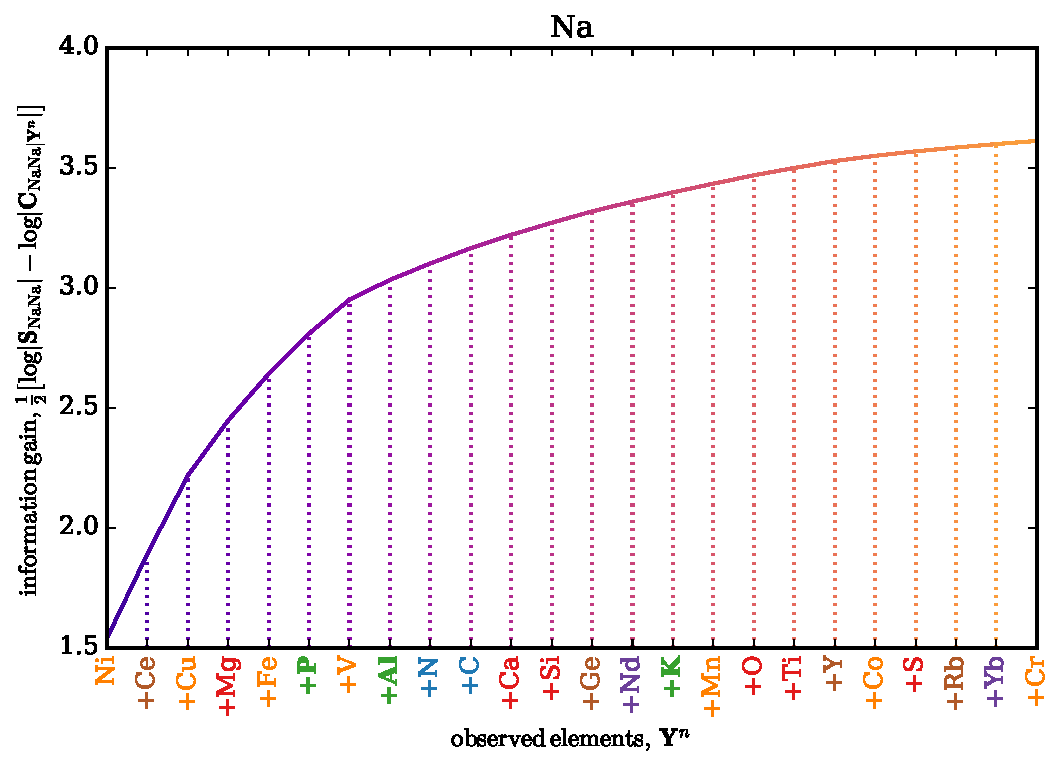
\includegraphics[width=\columnwidth]{apogee_centers_final_29502_spc_win_wid_1p5_na_inf_gain.pdf}
	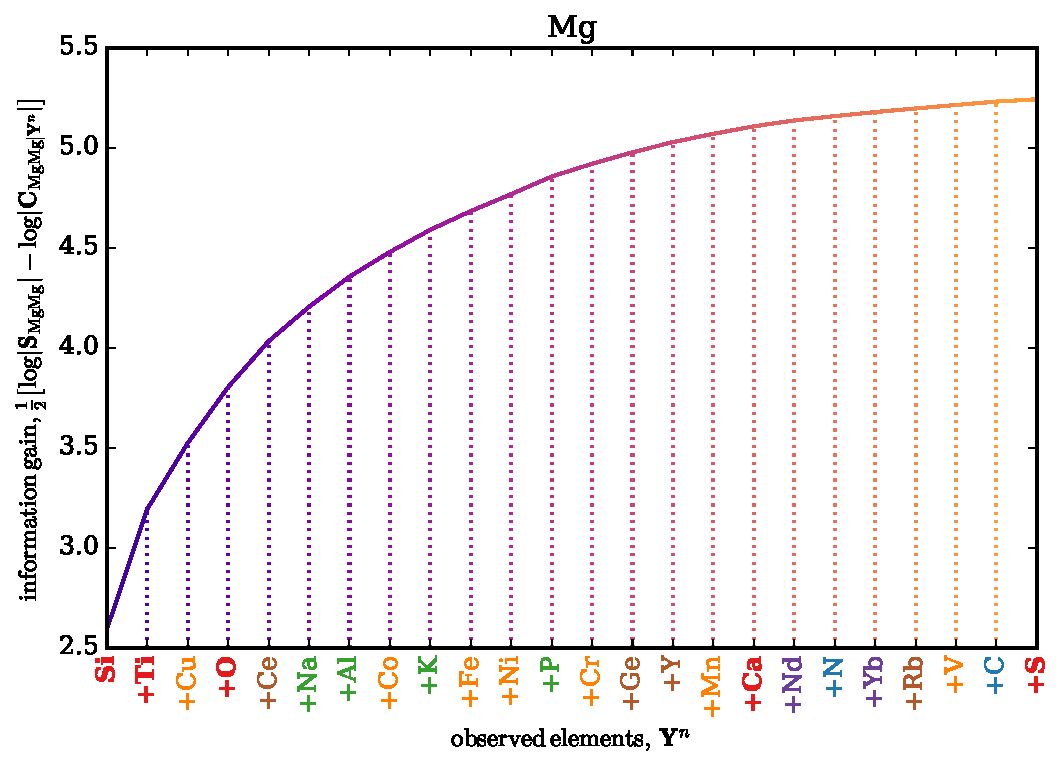
\includegraphics[width=\columnwidth]{apogee_centers_final_29502_spc_win_wid_1p5_mg_inf_gain.pdf}
	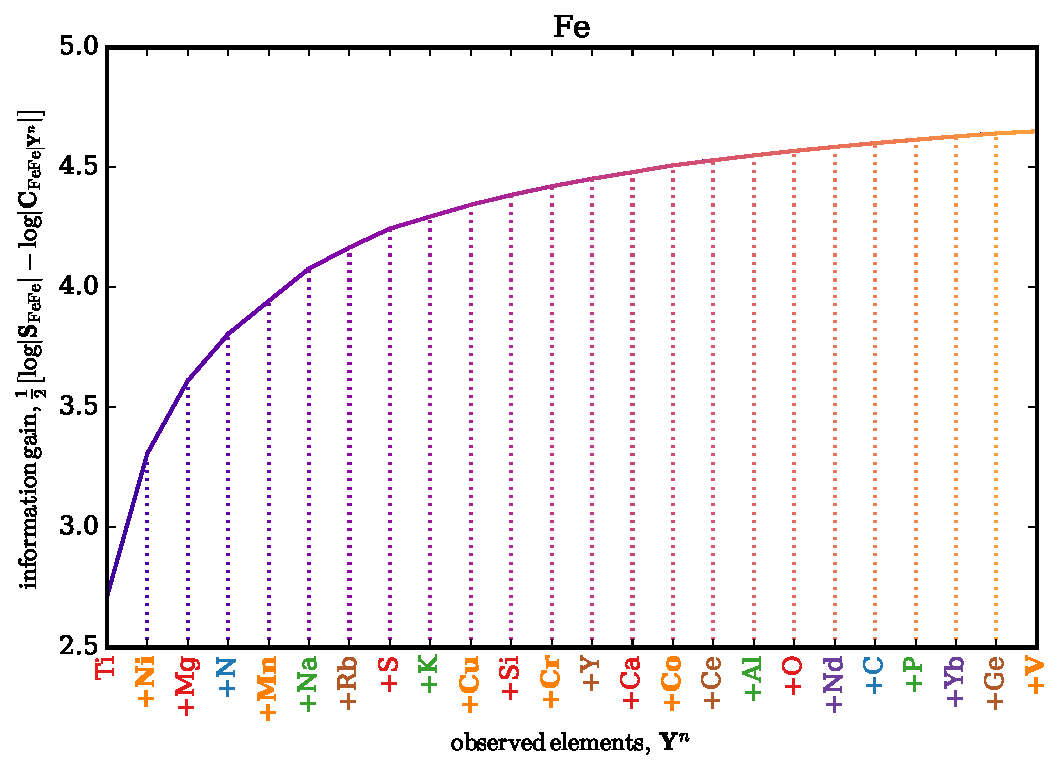
\includegraphics[width=\columnwidth]{apogee_centers_final_29502_spc_win_wid_1p5_fe_inf_gain.pdf}
	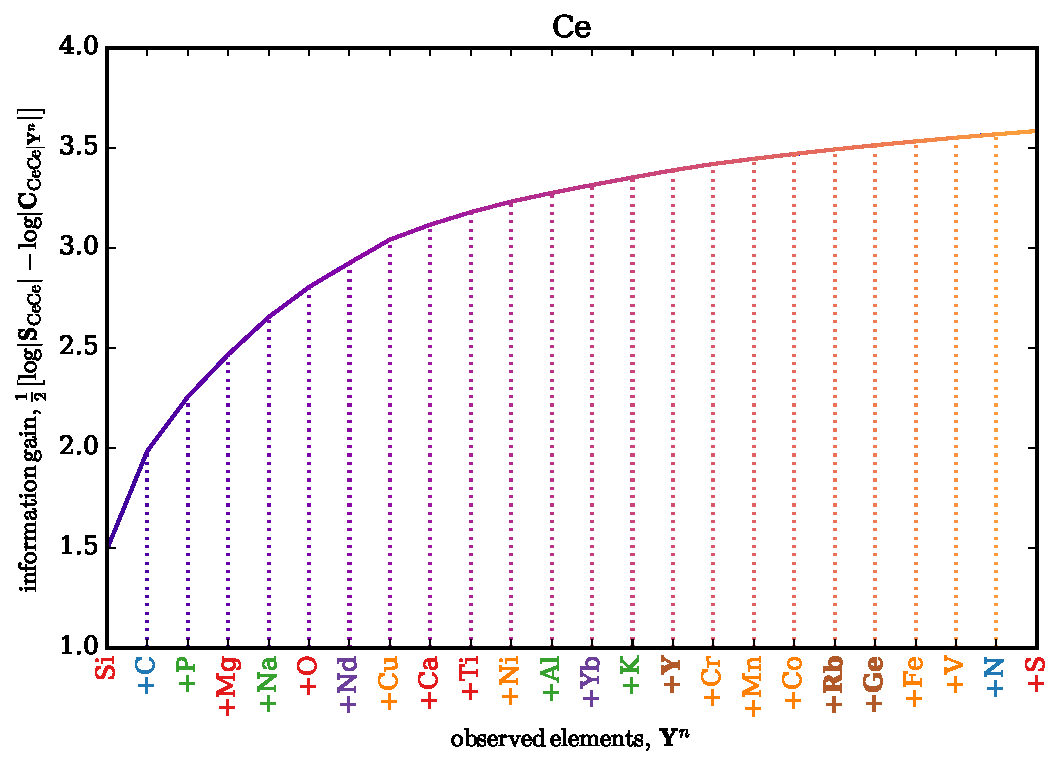
\includegraphics[width=\columnwidth]{apogee_centers_final_29502_spc_win_wid_1p5_ce_inf_gain.pdf}
	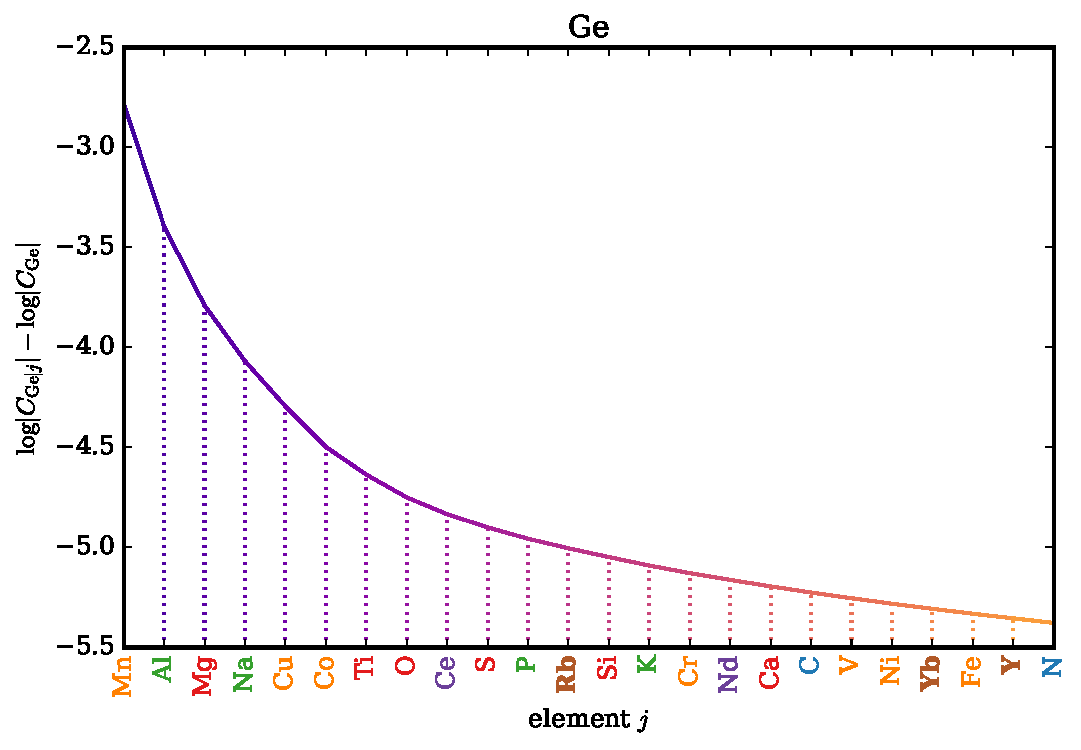
\includegraphics[width=\columnwidth]{apogee_centers_final_29502_spc_win_wid_1p5_ge_inf_gain.pdf}
    \caption{These set of figures represent the information gains for the windows corresponding to the elements C, Na, Mg, Fe, Ce and Ge, as shown in the top of each sub-panel, given observations of the other 24 elemental windows. Each of the element windows is shown on the x-axis, ordered from the most informative window with respect to the primary selected element, that remains after conditioning on all previous element windows. To take the top right-hand sub-panel as an example: one would learn the most about the C window by observing Ni, then adding Ce, Ti {\it et cetera}. The y-axis quantifies this predictivity of successive elements as a measure of information gain, which is the change in entropy of the system provided by conditioning on another piece of information. Note the changing range in scale of the measure of information gain for the six different elements. The gain of the 24 additional element windows in the example of the the C primary window is less than the information gain for the Na primary windows. A larger overall difference is indicative of a larger overall information gain by measuring more elements. Note that the near exponential element-information gain relation, while becoming far less steep, does not entirely flatten, which indicates that each single element adds additional information to learn about the primary element. Although elements are highly correlated, there is a small intrinsic variance in each element that is not predicted in full by the remaining set of windows. }
    \label{fig:single_element_information}
\end{figure*}

% most predictive
% y axis quantifes the information gain. 
%the information gain is defined here as the difference between the log of the ratio of the determinant of the covariance matrix conditioned on observation in some other window and divided by the covariance matrix not condioned on any other obsservation. 
%log of the determinant of the covariance matirx tells  you the change in entropy of the system that you would get by conditioning on another piece of information.
% so it is very much an amoutn of information.
%low dimensional to some threshold
%two things - not looking at single elemental abundances because there might be other stuff in those windows, we are not using the same basis as abundances. Even if we were looking at abundances, not perfectly predictive. 
%intrinsic variance is coming out in this figure. 

\begin{figure*}
	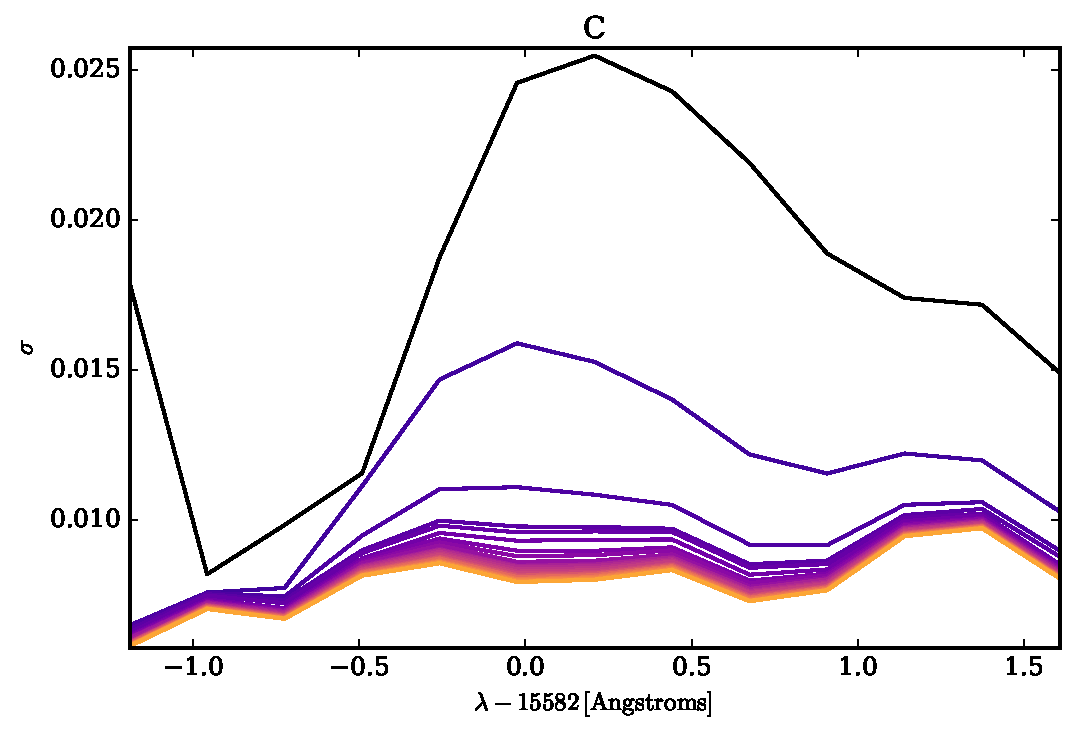
\includegraphics[width=\columnwidth]{apogee_centers_final_29502_spc_win_wid_1p5_c_conditional_stddevs.pdf}
	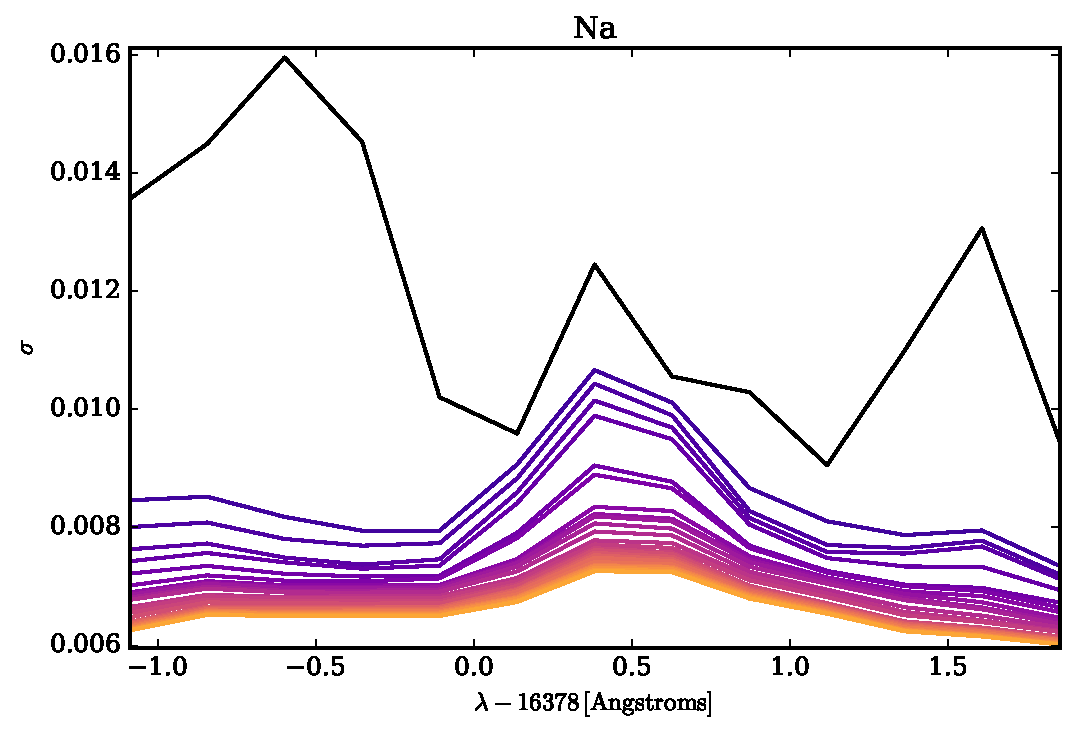
\includegraphics[width=\columnwidth]{apogee_centers_final_29502_spc_win_wid_1p5_na_conditional_stddevs.pdf}
	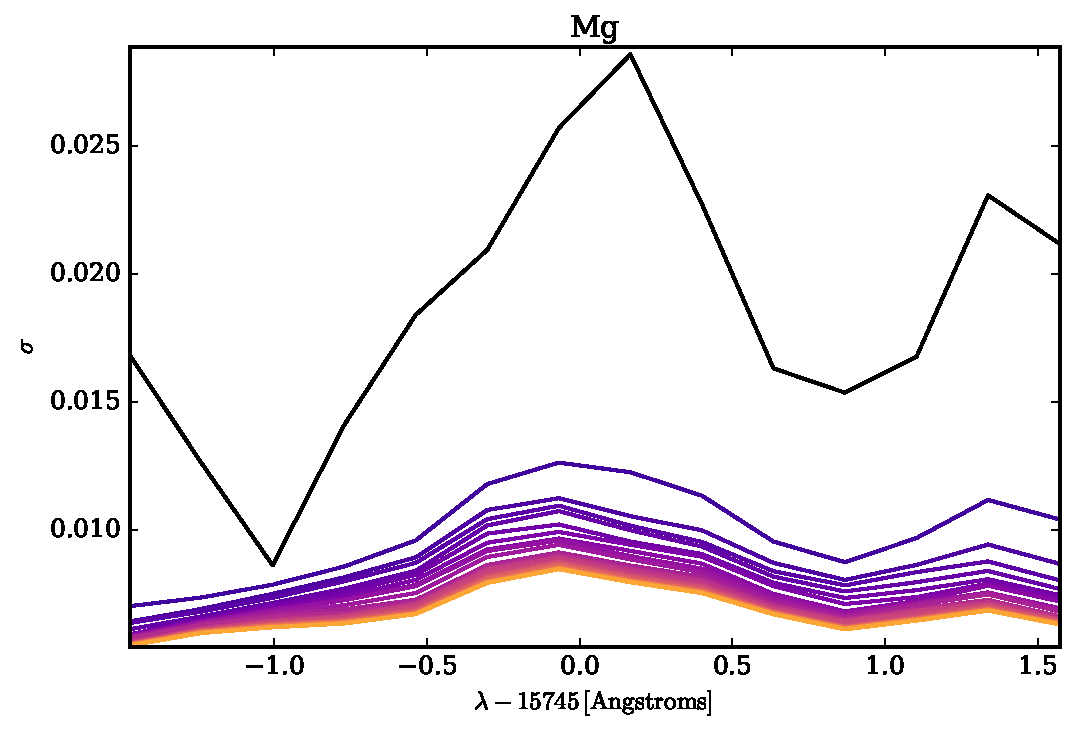
\includegraphics[width=\columnwidth]{apogee_centers_final_29502_spc_win_wid_1p5_mg_conditional_stddevs.pdf}
	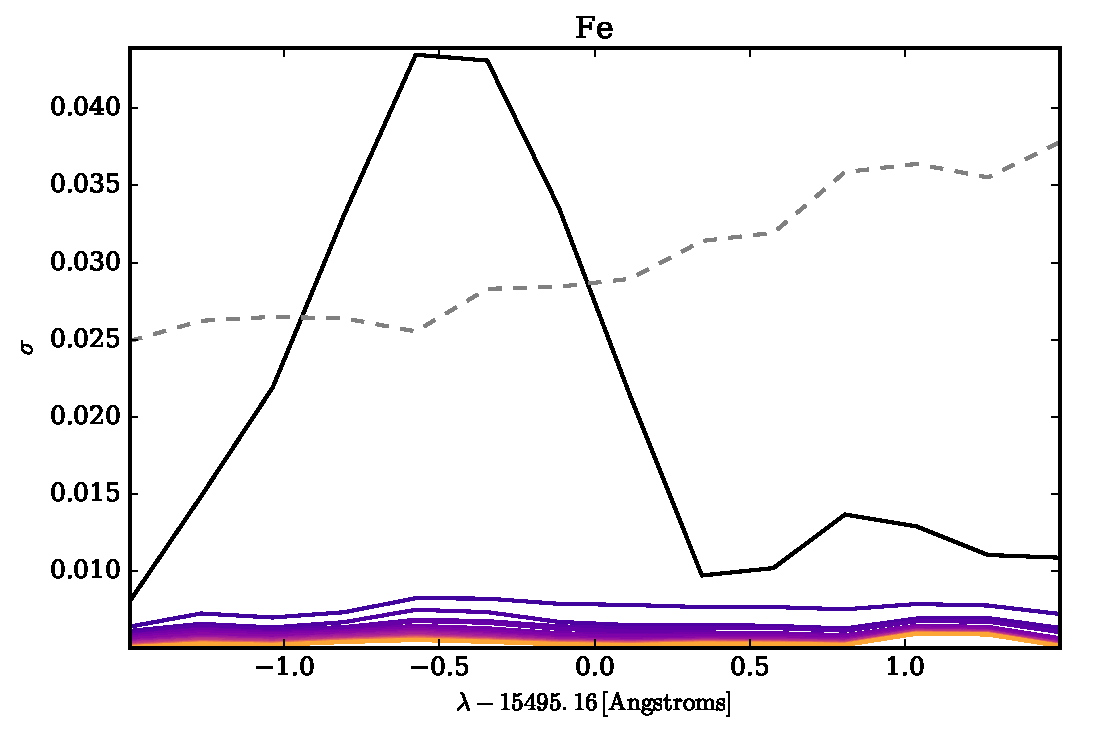
\includegraphics[width=\columnwidth]{apogee_centers_final_29502_spc_win_wid_1p5_fe_conditional_stddevs.pdf}
	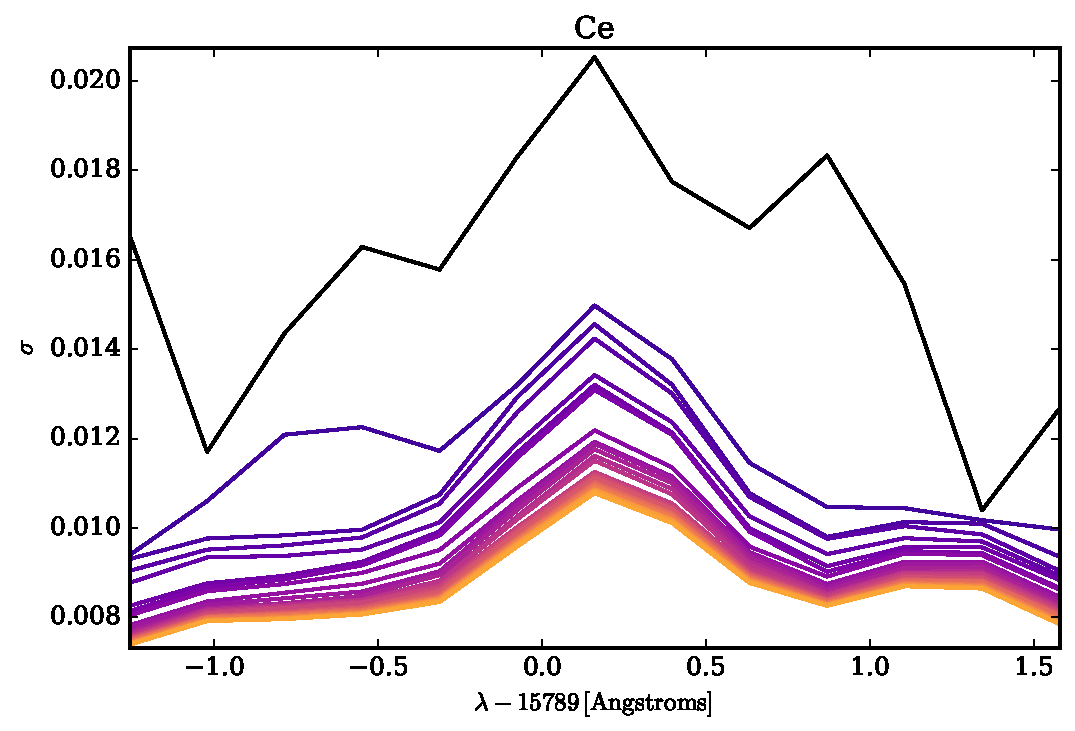
\includegraphics[width=\columnwidth]{apogee_centers_final_29502_spc_win_wid_1p5_ce_conditional_stddevs.pdf}
	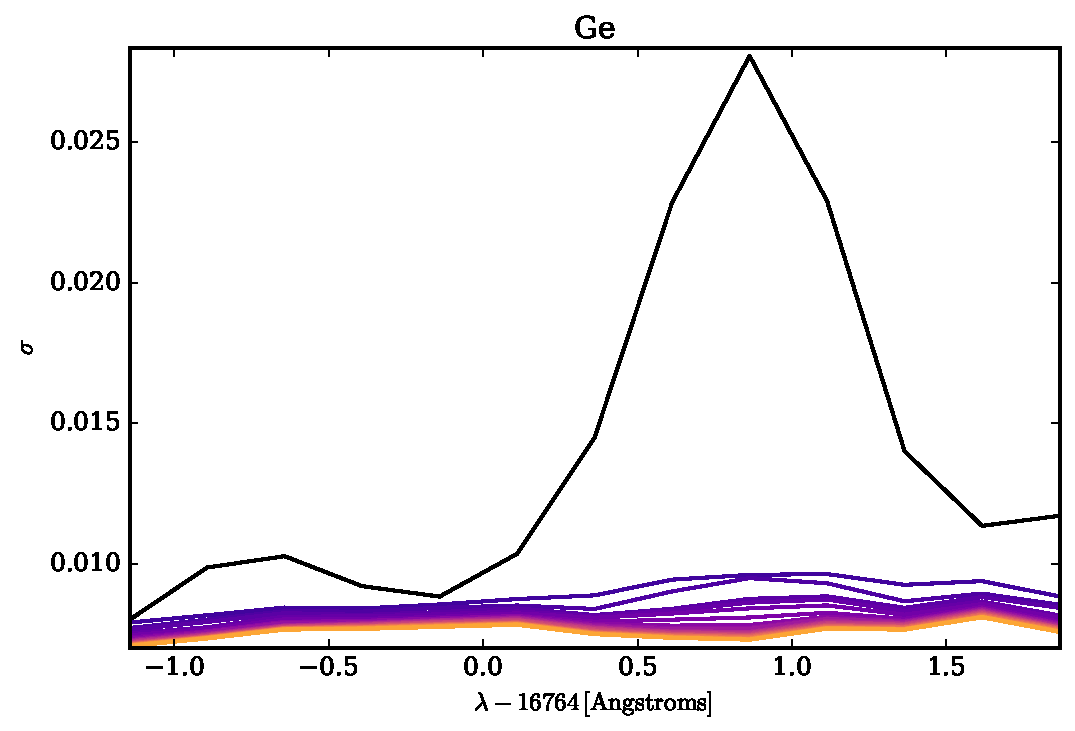
\includegraphics[width=\columnwidth]{apogee_centers_final_29502_spc_win_wid_1p5_ge_conditional_stddevs.pdf}
    \caption{These six sub-panels correspond to the same element windows as shown in Figure 6 of C, Na, Mg, Fe, Ce and Ge, as indicated in the top of each panel. In this Figure, the x-axis is centered on the wavelength of each primary element and the y-axis shows the conditional standard deviations for our  given observations of other elemental windows, added in the order set out in the corresponding panel of Fig.~\ref{fig:single_element_information}. The black line shows the uncertainty on the predicted spectrum without observations of other windows. The remaining 24 lines then correspond to the element windows ordered on the x-axis of the corresponding sub-panels of Fig.~\ref{fig:single_element_information}, from the most to least informative element window. This corresponds to the highest, in purple, to lowest, in yellow uncertainties on the predicted spectrum as each additional element is added. Note the uncertainties decrease less as the element-information gain relation becomes less steep in Fig.  Fig.~\ref{fig:single_element_information}. \textcolor{blue}{Now centered on the window center, with the average noise (of unmasked spectra) overlaid as a grey dashed line.}}
    \label{fig:single_element_errs}
\end{figure*}
%for each pixel shows the variance
%mean covariance matrix 
% in the order of figure 6 and coloured from black to yellow. All 24 are there. 
%centered on the nearest integer wavelength to the line center 

\begin{figure*}
	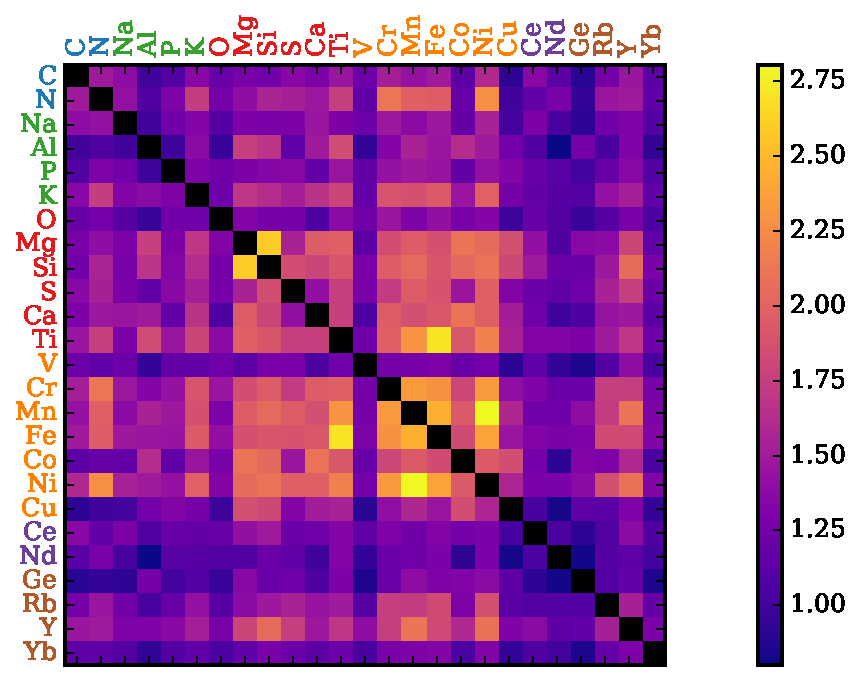
\includegraphics[width=\columnwidth]{apogee_centers_final_29502_spc_win_wid_1p5_sorted_inf_gains_fam_z.pdf}
	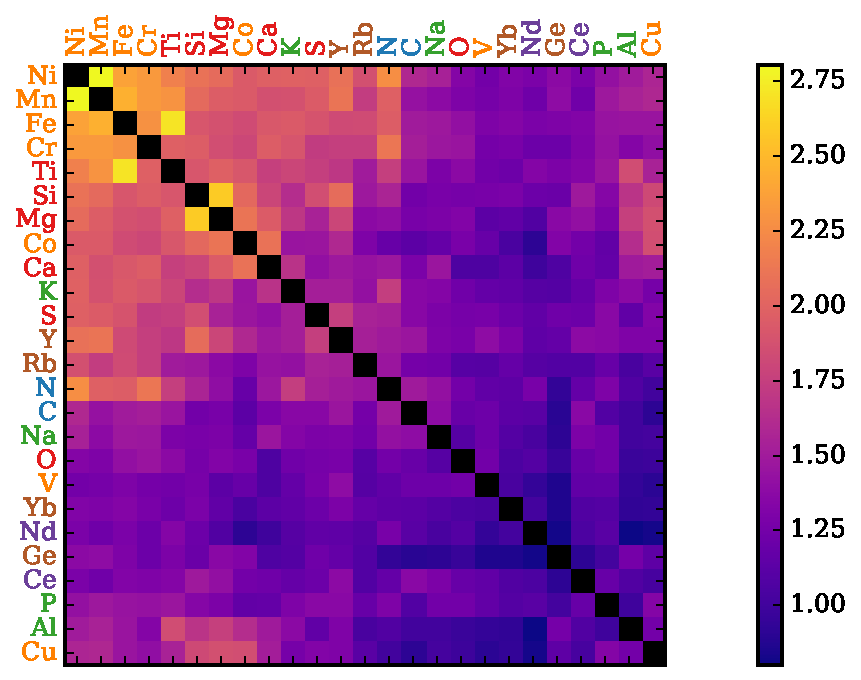
\includegraphics[width=\columnwidth]{apogee_centers_final_29502_spc_win_wid_1p5_sorted_inf_gains_abs_min_tot_dist.pdf}
    \caption{These two matricies show the information gains for pairs of elemental windows where a more negative measure represents a higher information gain. The information gain shown in the colourbar is defined as per  Fig.~\ref{fig:single_element_information}. Therefore, the brighter (more yellow) the matrix element, the more informative the windows are about each other. At left, the elements are grouped according to their nucleosynthetic family, indicated by label colour of the elements listed on the x and y axes (see the text). \textcolor{blue}{mkn: add a description to the text of the different families and what color they appear in}. At right, the elements are grouped by their similar information gain. Note that the iron-peak family of elements shows the highest paired information gains confined within this family (Ni, Mn, Fe, Cr) - these elements are most predictive of one another, followed by the alpha-element family of elements (Ti, Si, Mg). However, the ordering of elements by their information gain similarity does not discretely separate elements into their nucleosynthetic families, particularly beyond the iron-peak and alpha-elements. {mkn: make sure to put in the text that this is windows and sensitive to whatever else is in there as not abudanance measurement, so need to be clear about being about windows and not a discrete measurement of abundance correlation etc.}. Information gains for all pairs of elemental windows: the brighter the matrix element, the more informative the windows are about each other. Left: elements grouped according to their family, indicated by label colour. Right: elements grouped by similar information gains.}
    \label{fig:single_element_errs}
\end{figure*}

\begin{figure}
	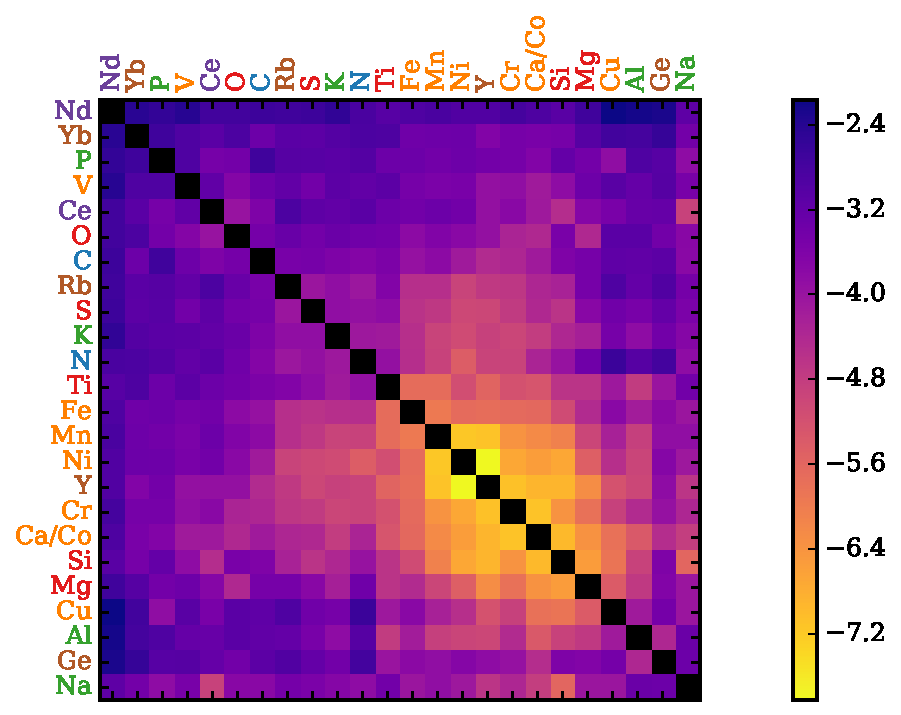
\includegraphics[width=\columnwidth]{apogee_centers_final_29502_spc_sorted_inf_gains_abs_min_tot_dist.pdf}
    \caption{This Figure is the same as the right hand panel of Figure 8 (with elements grouped by similar information gains) except using wider 5 \AA windows, compared to the 3 \AA\ windows in Figure 8.  This Figure highlights the sensitivity of the information gain to the bandwidth selected to indicate each element in determination of which elements are most similar to one another. Although the similarity ranking has changed, the iron peak elements remain grouped as before and two of the alpha-elements (Mg and Si) are adjacent, as previously.\textcolor{blue}{mkn: make sure to highlight this aspect of our analysis in the text, that we show that we can denoise spectra for abundance measurements but here using the pixels themselves not isolated abundances to examine correlations and information, which is totally legitimate and useful just need to come back to this. }}
    \label{fig:single_element_errs_wide}
\end{figure}

%through similarity

%%%%%%%%%%%%%%%%%%%%%%%%%%%%%%%%%%%%%%%%%%%%%%%%%%

\section{Conclusions}

TBD.

%%%%%%%%%%%%%%%%%%%%%%%%%%%%%%%%%%%%%%%%%%%%%%%%%%

\section*{Acknowledgements}

The Flatiron Institute is supported by the Simons Foundation.

%%%%%%%%%%%%%%%%%%%%%%%%%%%%%%%%%%%%%%%%%%%%%%%%%%

%\bibliographystyle{mnras}
%\bibliography{example} % if your bibtex file is called example.bib

%%%%%%%%%%%%%%%%%%%%%%%%%%%%%%%%%%%%%%%%%%%%%%%%%%


% Don't change these lines
\bsp	% typesetting comment
\label{lastpage}
\end{document}

% End of mnras_template.tex